\chapter{Detailed design}
\label{chap:detDesign}


Provide an introduction to the proposed design. This introduction should help
the reader to understand the design choices made.


\section{Interaction Model}
An Interaction Model describes how each \gls{system operation} (that appears in the
Operation Model of the \msrmessir Requirements Analysis Model) is designed to meet
its specification. The design description of each system operation must be
focused on the messages exchanged between the different first-class objects
(i.e. instances of classes either included in Concept Model or introduced as
result of a design choice). An Interaction Model is modeled as a UML Sequence
Diagram.


\subsection{oeSetClock}
An active message used to statically set the date and time information in the
systems state.

\begin{figure}[H]
\begin{center}
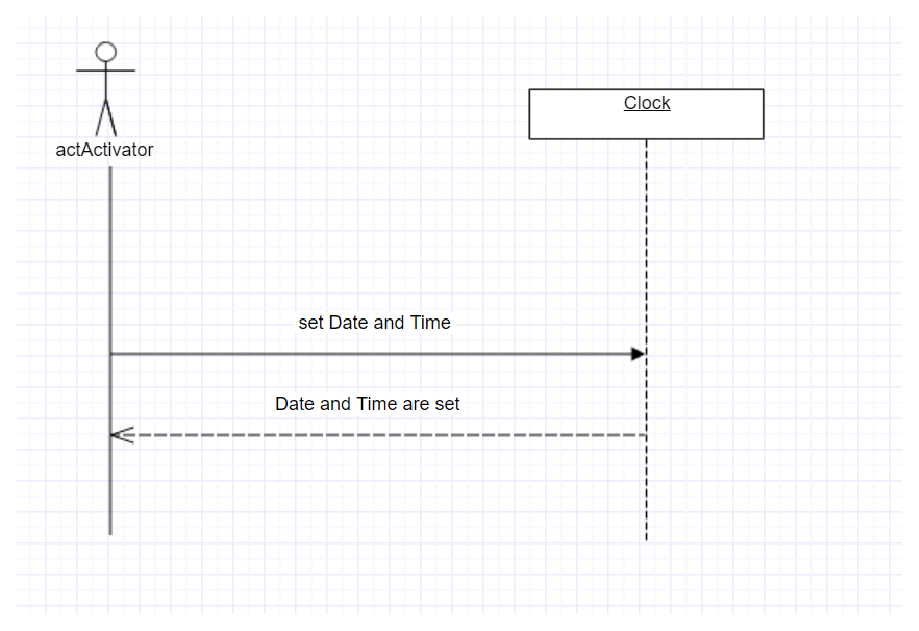
\includegraphics[width=0.5\textwidth]{./images/oeSetClock.eps} 
\end{center}
\caption{oeSetClock}
\end{figure}


\subsection{oeSollicitateCrisisHandling}
A proactive message (message of a pro-active actor with no parameter triggered
automatically if the pre protocol condition is true) used to avoid crisis to
stay too long in an not handled status
\begin{figure}[H]
\begin{center}
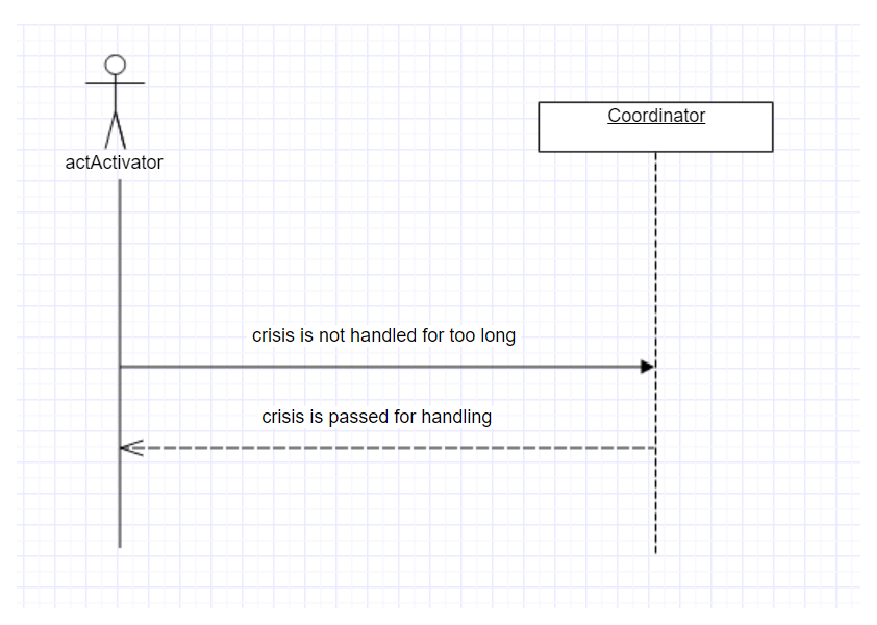
\includegraphics[width=0.5\textwidth]{./images/oeSollicitateCrisisHandling.eps} 
\end{center}
\caption{oeSollicitateCrisisHandling}
\end{figure}


\subsection{oeAddCoordinator}
Sent to add a new coordinator in the systems post state and environments post
state.
\begin{figure}[H]
\begin{center}
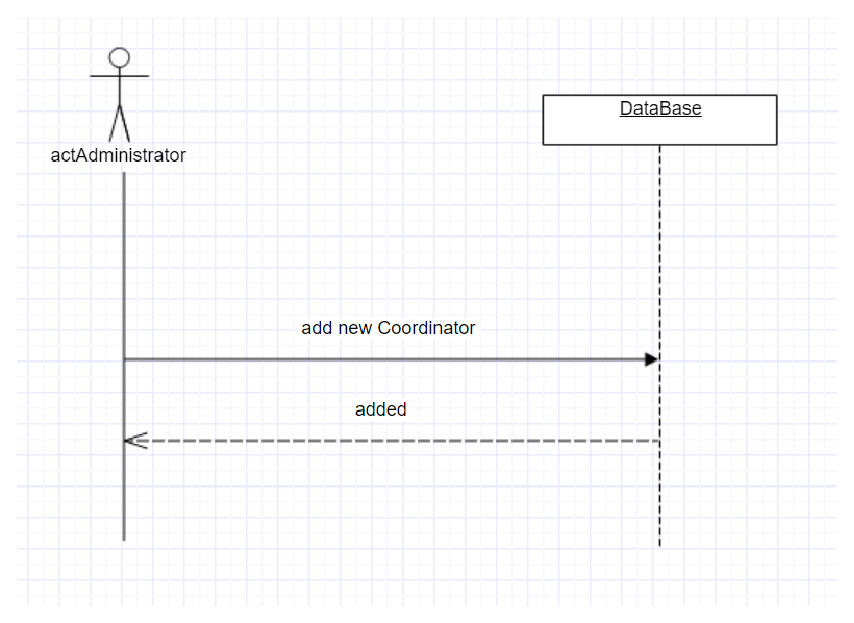
\includegraphics[width=0.5\textwidth]{./images/oeAddCoordinator.eps} 
\end{center}
\caption{oeAddCoordinator}
\end{figure}


\subsection{oeDeleteCoordinator}
Sent to delete an existing coordinator in the systems post state and
environments post state.
\begin{figure}[H]
\begin{center}
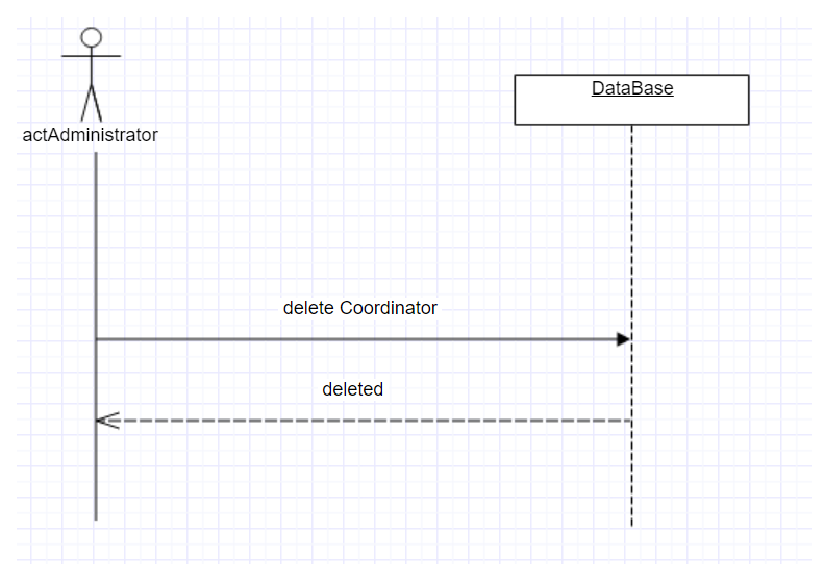
\includegraphics[width=0.5\textwidth]{./images/oeDeleteCoordinator.eps} 
\end{center}
\caption{oeDeleteCoordinator}
\end{figure}

\subsection{oeLogin}
Sent to request authorization to request access secured system operations.
\begin{figure}[H]
\begin{center}
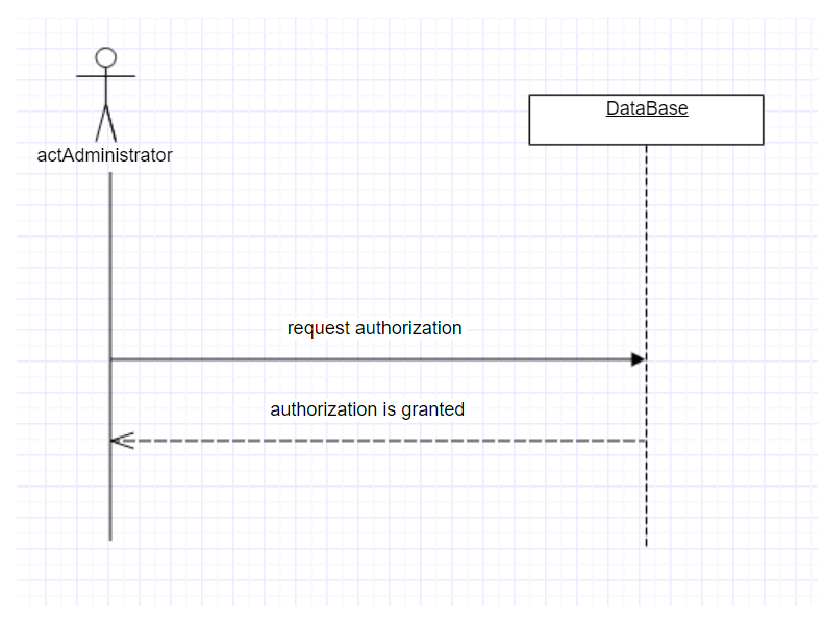
\includegraphics[width=0.5\textwidth]{./images/oeLogin.eps} 
\end{center}
\caption{oeLogin}
\end{figure}

\subsection{oeLogout}
Sent to end the secured access to specific system operations

\begin{figure}[H]
\begin{center}
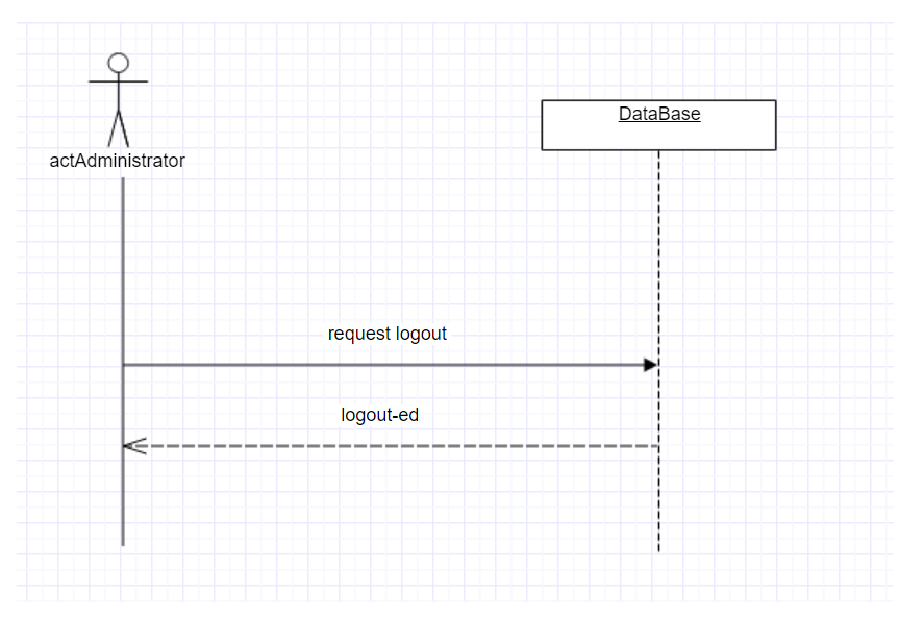
\includegraphics[width=0.5\textwidth]{./images/oeLogout.eps} 
\end{center}
\caption{oeLogout}
\end{figure}

\subsection{oeAlert}
Any human having a phone able to connect to the communication companies using
the iCrash system can send his company an sms message with structured
information in order to declare an alert

\begin{figure}[H]
\begin{center}
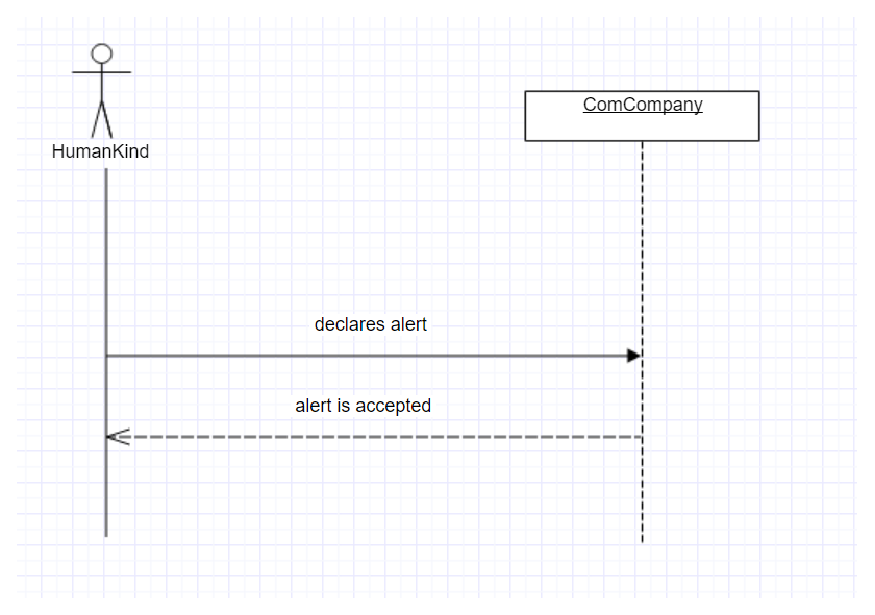
\includegraphics[width=0.5\textwidth]{./images/oeAlert.eps} 
\end{center}
\caption{oeAlert}
\end{figure}

\subsection{oeCloseCrisis}
Sent to indicate that a crisis should be considered as closed.

\begin{figure}[H]
\begin{center}
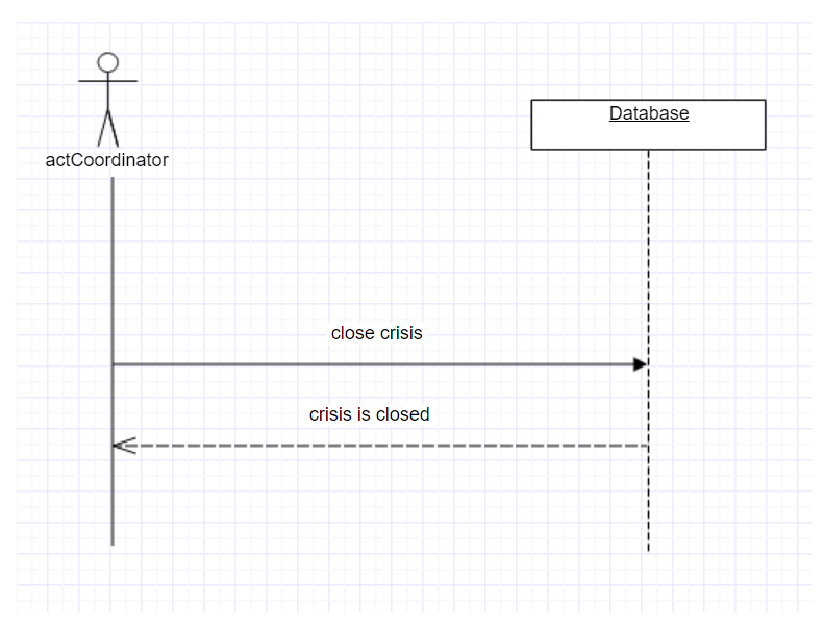
\includegraphics[width=0.5\textwidth]{./images/oeCloseCrisis.eps} 
\end{center}
\caption{oeCloseCrisis}
\end{figure}

\subsection{oeGetAlertsSet}
Sent to request all the ctAlert instances having a specific status.

\begin{figure}[H]
\begin{center}
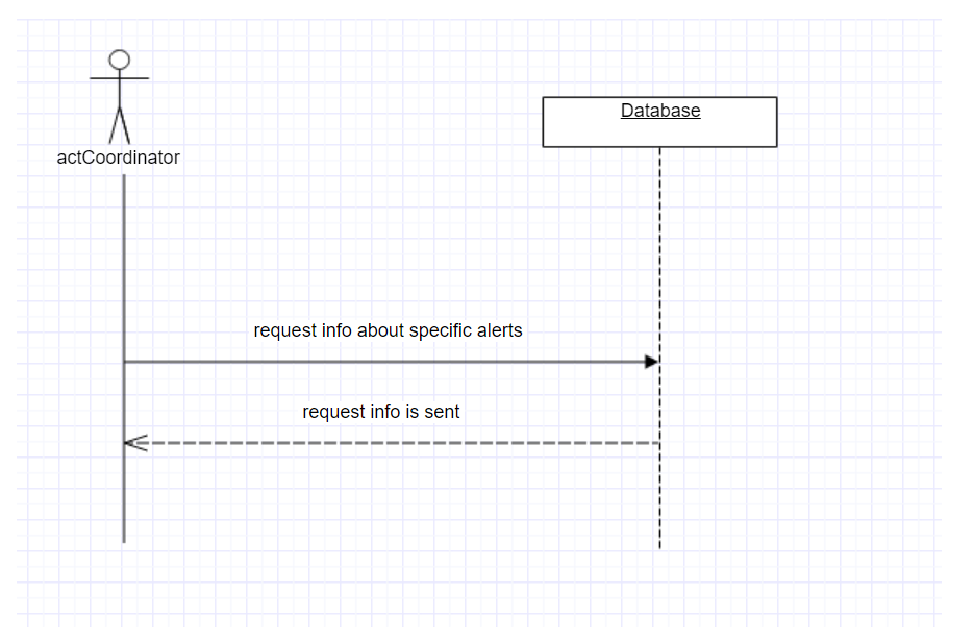
\includegraphics[width=0.5\textwidth]{./images/oeGetAlertsSet.eps} 
\end{center}
\caption{oeGetAlertsSet}
\end{figure}

\subsection{oeGetCrisisSet}
Sent to request all the ctCrisis instances having a specific status.

\begin{figure}[H]
\begin{center}
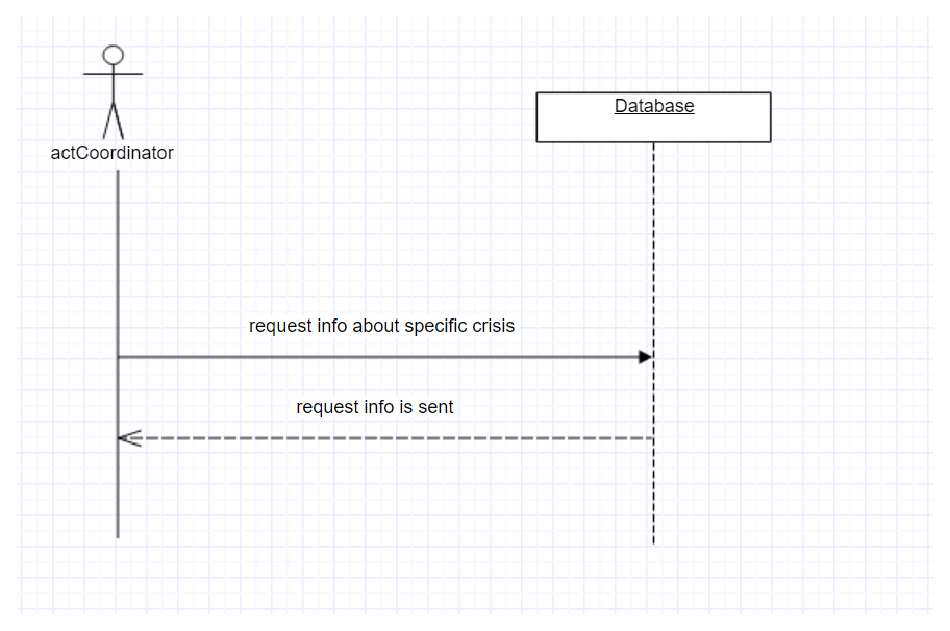
\includegraphics[width=0.5\textwidth]{./images/oeGetCrisisSet.eps} 
\end{center}
\caption{oeGetCrisisSet}
\end{figure}

\subsection{oeInvalidateAlert}
Sent to indicate that an alert should be considered as closed.

\begin{figure}[H]
\begin{center}
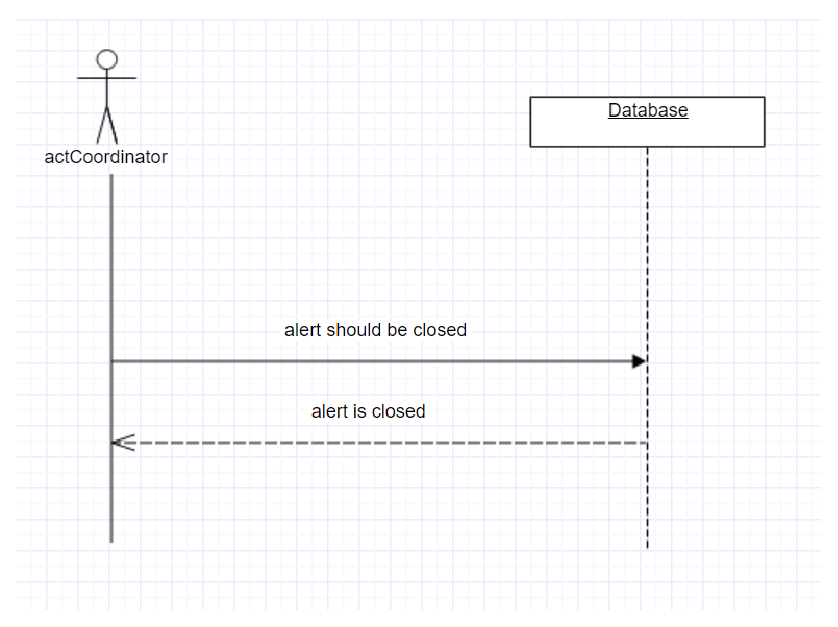
\includegraphics[width=0.5\textwidth]{./images/oeInvalidateAlert.eps} 
\end{center}
\caption{oeInvalidateAlert}
\end{figure}

\subsection{oeReportOnCrisis}
Sent to update the textual information available for a specific handled crisis.

\begin{figure}[H]
\begin{center}
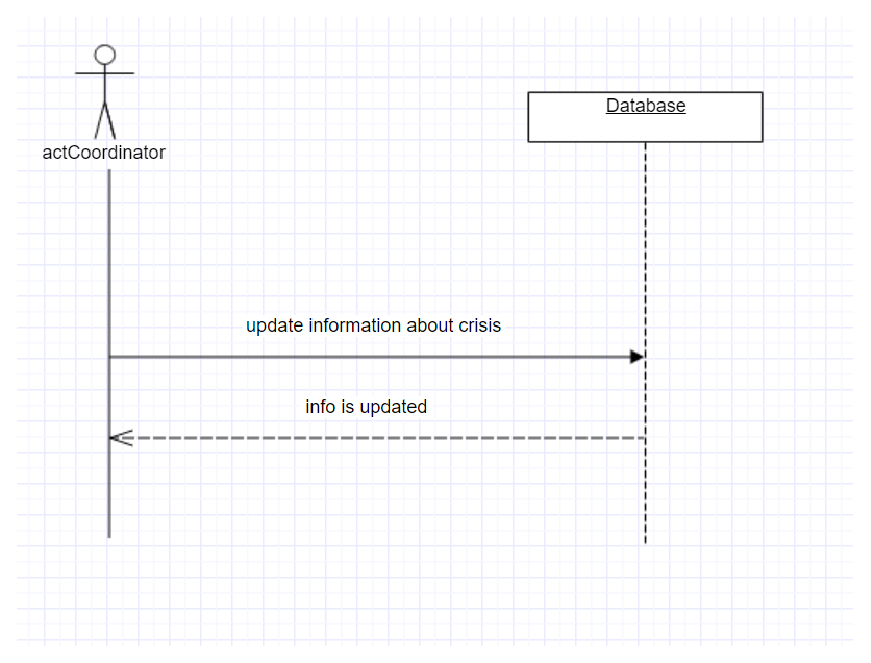
\includegraphics[width=0.5\textwidth]{./images/oeReportOnCrisis.eps} 
\end{center}
\caption{oeReportOnCrisis}
\end{figure}

\subsection{oeSetCrisisHandler}
Sent to declare himself as been the handler of a crisis having the specified id

\begin{figure}[H]
\begin{center}
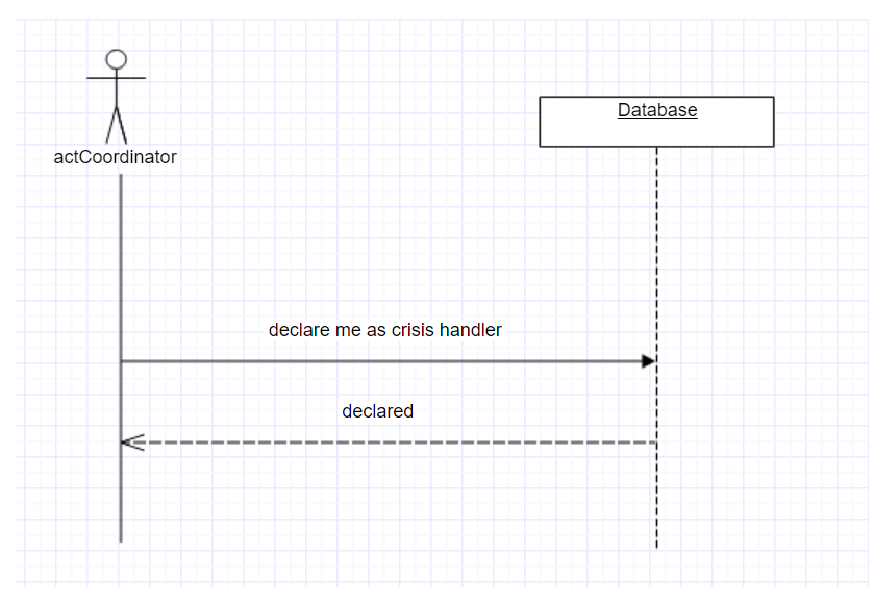
\includegraphics[width=0.5\textwidth]{./images/oeSetCrisisHandler.eps} 
\end{center}
\caption{oeSetCrisisHandler}
\end{figure}

\subsection{oeCreateSystemAndEnvironment}
oeCreateSystemAndEnvironment sent to request the initialization of the systems
class instances and the environment actors instances.

\begin{figure}[H]
\begin{center}
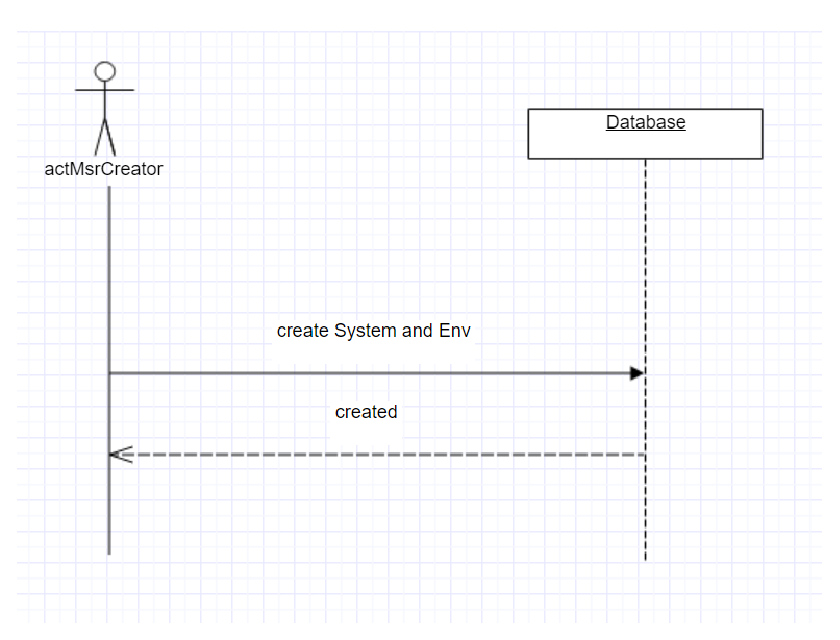
\includegraphics[width=0.5\textwidth]{./images/oeCreateSystemAndEnvironment.eps} 
\end{center}
\caption{oeCreateSystemAndEnvironment}
\end{figure}

\subsection{init}
init used to create an instance of the actor together with its interface
instances and update the assocations with the ctState instance.

\begin{figure}[H]
\begin{center}
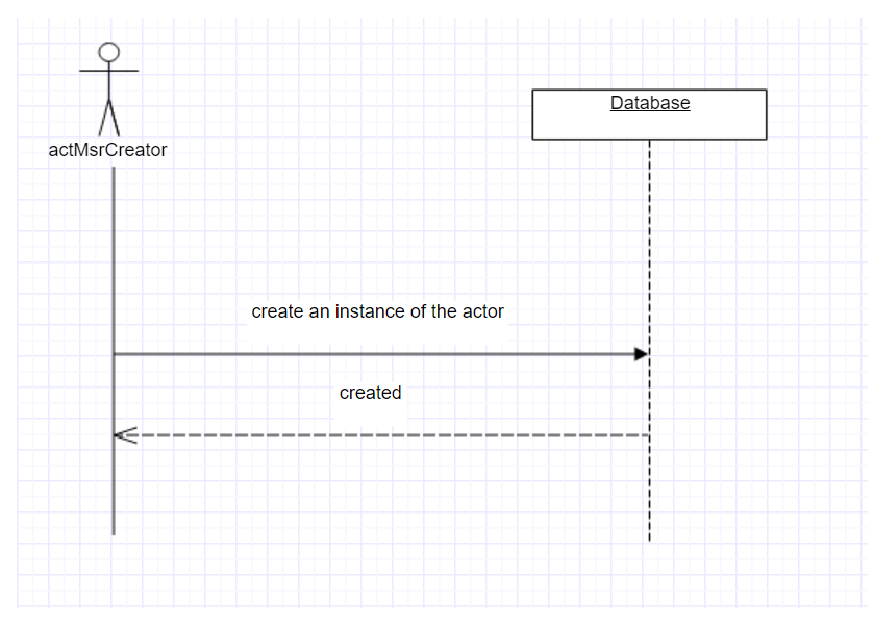
\includegraphics[width=0.5\textwidth]{./images/init.eps} 
\end{center}
\caption{init}
\end{figure}




\section{Design Class Model}
The Design Class Model is composed of the contents of all design classes (i.e.
every class appearing in at least one Interaction Model), all the navigable associations between design
classes, and the inheritance structure. The description of each class must
contain its attributes and operations. The Design Class Model is modeled as a
UML Class Diagram. 

It is advised to split the Design Class Model into multiple views as such model
may become pretty large. 
	

\subsection{Design Class Model view1}
TODO


\subsection{Design Class Model view2}
TODO



\subsection{Design Class Model view3}
TODO